\input ../SlidePreamble
\input ../preamble


\begin{document}

{\Huge

  \centerline{\bf TTIC 31230, Fundamentals of Deep Learning}
  \bigskip
  \centerline{David McAllester, Winter 2018}
  \vfill
  \centerline{\bf Deep Graphical Models II}
  \vfill
  \centerline{\bf Algorithms for Approximate SGD}
  \vfill
  \centerline{MCMC Sampling}
  \vfill
  \centerline{Pseudo-Likelihood}
  \vfill
  \centerline{Contrastive Divergence}
\vfill

\slide{Superpixel Colorization}

\centerline{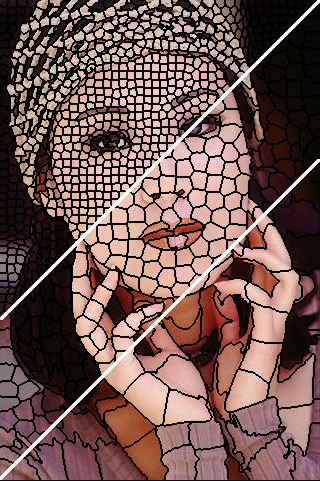
\includegraphics[height = 3in]{../images/SLIC} \hspace{.5in} 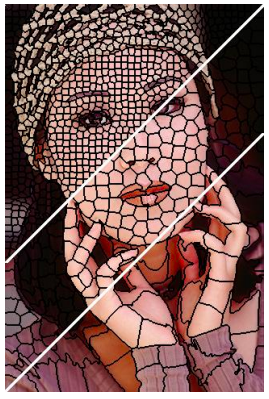
\includegraphics[height = 3in]{../images/SLICcolor}}
\centerline{\huge SLIC superpixels, Achanta et al.}

$x$ is a black and white image.

\vfill
$y$ is a color image drawn from $\pop(y|x)$.

\vfill
$\hat{y}$ is an arbitrary color image.

\vfill
$P_\Phi(\hat{y}|x)$ is the probability that model $\Phi$ assigns to the color image $y$ given black and white image $x$.

\slideplain{Exponential Softmax}

The tensor $s_e[\tilde{y}]$ is computed from $x$ and $\Phi$.

\vfill
\begin{eqnarray*}
P_s(\hat{y}) & = &\softmax_{\hat{y}}\;s(\hat{y}) \\
\\
s(\hat{y}) & = & \sum_{e \in \mathrm{HyperEdges}}  \; s_e[\hat{y}[e]]
\end{eqnarray*}

\slide{Backpropagation}

The input is the image $x$ and the parameter package $\Phi$

\begin{eqnarray*}
 & \vdots & \\
s_e[\hat{y}] & = & \ldots \\
{\cal L} & = & - \ln\; P(y\;|\;s_{\cal E}[{\cal Y}])
\end{eqnarray*}

\vfill We abbreviate $P(\hat{y}\;|\;s_{\cal E}[{\cal Y}])$ as {\color{red} $P_s(\hat{y})$} --- the distribution on $\hat{y}$ defined by the tensor $s$.
\vfill
We need to compute {\color{red} $\nabla_s -\ln P_s(y)$}, or equivalently, {\color{red} $s_e.\grad[\tilde{y}]$}.

\begin{eqnarray*}
s_e.\mathrm{grad}[\tilde{y}] & = &  {\color{red} P_e(\tilde{y})} - \bbone[\tilde{y} = y[e]]
\end{eqnarray*}


\slide{Sampling}
The quantities ${\color{red} P_e(\tilde{e})}$ are {\bf hyperedge marginals}.

\vfill
We can estimate the hyperedge marginals by sampling $\hat{y}$ from $P_s(\hat{y})$.

\slide{Monte Carlo Markov Chain (MCMC) Sampling}

\centerline{\bf Metropolis Algorithm}

\vfill
Pick an initial graph label $\hat{y}$ and then repeat:

\begin{enumerate}
\item Pick a ``neighbor'' $\hat{y}'$ of $\hat{y}$ uniformly at random.  The neighbor relation must be symmetric.  Perhaps Hamming distance one.

  \vfill
\item If $s(\hat{y}') > s(\hat{y})$ update $\hat{y} = \hat{y}'$

  \vfill
\item If $s(\hat{y}') \leq s(\hat{y})$ then update $\hat{y} = \hat{y}'$ with probability $e^{-(s(\hat{y}) - s(\hat{y}'))}$
  \end{enumerate}  

\slide{Markov Processes and Stationary Distributions}

A Markov process is a process defined by a fixed state transition probability $P(\hat{y}'|\hat{y}) = M_{\hat{y}',\hat{y}}$.

\vfill
Let $P^t$ the probability distribution for time $t$.

\vfill
$$P^{t+1} = MP^t$$

\vfill
If every state can be reached form every state (ergodic process) then $P^t$ converges to a unique {\bf stationary distribution} $P^\infty$

\vfill
$$P^\infty = MP^\infty$$

\slide{Metropolis Correctness}

To verify that the Metropolis process has the correct stationary distribution we simply verify that $MP = P$ where $P$
is the desired distribution.

\vfill
This can be done by checking that under the desired distribution the flow from $\hat{y}$ to $\hat{y}'$
equals the flow from $\hat{y}'$ to $\hat{y}$ ({\bf detailed balance}).

\slide{Metropolis Correctness}

For $s(\hat{y}) \geq s(\hat{y}')$

\vfill
\begin{eqnarray*}
  \mathrm{flow}(\hat{y}' \rightarrow \hat{y}) &  = & \frac{1}{Z}e^{s(\hat{y}')} \frac{1}{N} \\
  \\
\mathrm{flow}(\hat{y} \rightarrow \hat{y}') & = & \frac{1}{Z}e^{s(\hat{y})} \frac{1}{N} e^{-\Delta f} = \frac{1}{Z} e^{s(\hat{y}')} \frac{1}{N}
\end{eqnarray*}

\vfill
But detailed balance is not required in general (see Hamiltonian MCMC).

\slide{Gibbs Sampling}

The Metropolis algorithm wastes time by rejecting proposed moves.

\vfill
Gibbs sampling avoids this move rejection.

\vfill
In Gibbs sampling we select a node $i$ at random and change that node by drawing a new node value conditioned on the current values of the other nodes.

\slide{Gibbs Sampling}

\begin{eqnarray*}
  P_s(i=\tilde{y} \;|\;\hat{y}) & \doteq & P_s(\hat{y}[i] = \tilde{y}\;|\;\hat{y}[1],\ldots,\hat{y}[i-1],\hat{y}[i+1],\ldots,\hat{y}[I])
\end{eqnarray*}

\vfill
Markov Blanket Property:
$$P_s(i=\tilde{y} \;|\;\hat{y}) = P_s(i=\tilde{y} \;|\;\hat{y}[N(i)])$$
  
\vfill
Gibbs Sampling, Repeat:

\begin{itemize}
\item   Select $i$ at random

\item draw $\tilde{y}$ from $P_s(i = \tilde{y} \;|\;\hat{y})$

\item $\hat{y}[i] = \tilde{y}$
\end{itemize}

\slide{Gibbs Sampling}

Let $\hat{y}[i = \tilde{y}]$ be the assignment $\hat{y}'$ equal to $\hat{y}$ except $\hat{y}'[i] = \tilde{y}$.

\vfill
\begin{eqnarray*}
 P_s(i = \tilde{y} \;|\; \hat{y})  & = & \frac{P_s(\hat{y}[i] = \tilde{y})}{\sum_{\tilde{y}} P_s(\hat{y}[i] = \tilde{y})} \\
  \\
  \\
  & = & \frac{e^{s(\hat{y}[i = \tilde{y}])}}{\sum_{\tilde{y}} e^{s(\hat{y}[i = \tilde{y}])}}
\end{eqnarray*}

\slide{Correctness Proof}

$P_s(\hat{y})$ is a stationary distribution of Gibbs Sampling.

\vfill
\begin{itemize}
\item   Select $i$ at random

\item draw $\tilde{y}$ from $P_s(i = \tilde{y} \;|\;\hat{y})$

\item $\hat{y}[i] = \tilde{y}$
\end{itemize}


\vfill
The distribution before the update equals the distribution after the update.

\slide{Pseudolikelihood}

In Pseudolikelihood we replace the objective $- \log P_s(\hat{y})$ with the objective $- \log \tilde{Q}_s(\hat{y})$ where

\vfill
\begin{eqnarray*}
  \tilde{Q}_s(\hat{y}) & \doteq & \prod_i \;P_s(i = \hat{y}[i] \;|\;\hat{y}) \\
  \\
  \mathrm{loss}(f) & \doteq & - \log \tilde{Q}(y) \\
  \\
  s.\mathrm{grad}[e,\tilde{y}] & = & \sum_i - \partial \log P_s[i = \hat{y}[i] \;|\;\hat{y}] /\partial s[e,\tilde{y}]
\end{eqnarray*}


\slide{Pseudolikelihood Consistency}

$$\argmin_Q \; E_{y \sim \mathrm{Pop}} \;-\log \tilde{Q}(y) = \mathrm{Pop}$$

\vfill

\slide{Proof of Consistency I}

We have

$$\min_{Q} \;E_{y \sim \mathrm{Pop}}\;-\log \tilde{Q}(y) \;\;\leq \;\; E_{y \sim \mathrm{Pop}}\;-\log \widetilde{\mathrm{Pop}}(y)$$

\vfill
If we can show

$$\min_{Q} \;E_{y \sim \mathrm{Pop}}\;-\log \tilde{Q}(y) \;\;\geq \;\; E_{y \sim \mathrm{Pop}}\;-\log \widetilde{\mathrm{Pop}}(y)$$

Then the minimizer (the argmin) is $\mathrm{Pop}$ as desired.

\slide{Proof of Consistency II}

We will prove the case of two nodes.

\vfill
\begin{eqnarray*}
  & & \min_Q \;E_{y\sim \mathrm{Pop}}{-\log Q(y[1]|y[2])\;Q(y[2]|y[1])} \\
  \\
  & \geq & \min_{P_1,P_2} E_{y \sim \mathrm{Pop}}{-\log P_1(y[1]|y[2])\;P_2(y[2]|y[1])} \\
  \\
  & = & \min_{P_1} E_{y \sim \mathrm{Pop}}{-\log P_1(y[1]|y[2])} + \min_{P_2} E_{y \sim \mathrm{Pop}}{-\log P_2(y[2]|y[1])} \\
  \\
  & = & E_{y \sim \mathrm{Pop}}{-\log \mathrm{Pop}(y[1]|y[2])} + E_{y \sim \mathrm{Pop}}{-\log \mathrm{Pop}(y[2]|y[1])} \\
  \\
  & = & E_{y \sim \mathrm{Pop}}{-\log \widetilde{\mathrm{Pop}}(y|x)}
\end{eqnarray*}

  
\slideplain{Contrastive Divergence}
{\bf Algorithm (CDk)}: Run $k$ steps of MCMC for $P_s(\hat{y})$ {\bf starting from $y$} to get $\hat{y}$.

\vfill
Then set
$$s.\mathrm{grad}[e,\tilde{y}] = \mathbbm{1}[\hat{y}[e] = \tilde{y}] - \mathbbm{1}[y[e]= \tilde{y}]$$

\vfill
    {\bf Theorem}: If $P_s(\hat{y}) = \mathrm{Pop}$ then
    
    $$E_{y \sim \mathrm{Pop}}\; \mathbbm{1}[\hat{y}[e] = \tilde{y}] - \mathbbm{1}[y[e]= \tilde{y}] = 0$$

\vfill
{\bf Here we can take $k=1$ --- \bf no mixing time required}.


\slide{END}

}
\end{document}

